\begin{figure}
\centering
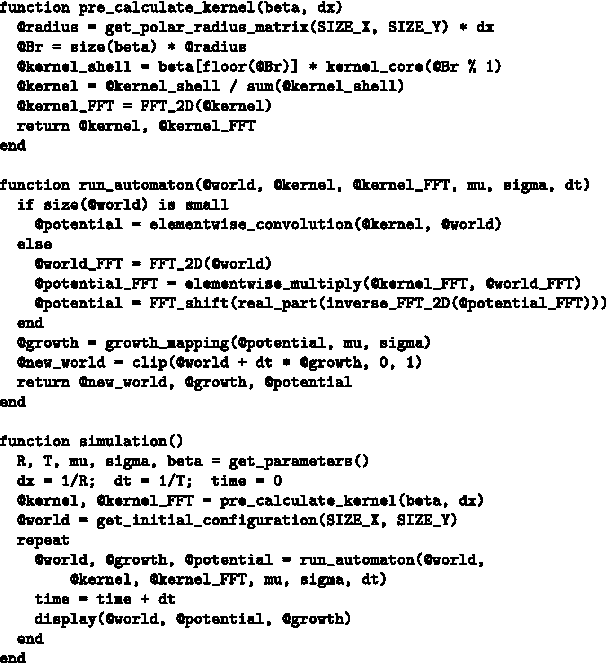
\includegraphics[width=0.5\textwidth]{img/lenia-pseudocode}
\caption{Pseudocde for Lenia update function, reproduced from \citep{chan2019lenia}.
Note that the use of a Fast Fourier Transform (FFT) is an optional optimization that leverages the frequency domain to perform convolution operations more efficiently on large operands, where direct element-wise convolution would be computationally intensive.
}
\label{fig:lenia-event-types}
\end{figure}
